\documentclass{article}

\usepackage{tikz}

\begin{document}

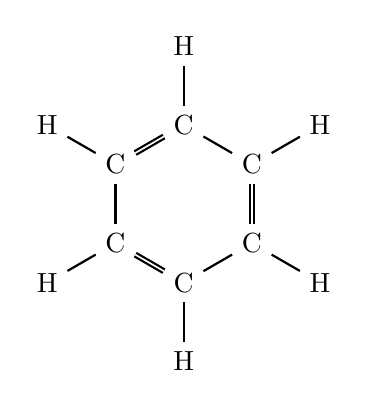
\begin{tikzpicture}
% les C et les H
\foreach \n/\a in {a/30,b/90,c/150,d/210,e/270,f/330}
    {\node (\n) at (\a:1) {C};
     \node (\n\n) at (\a:2) {H};}
    
% les liaisons C - H
\foreach \n in {a,b,c,d,e,f} \draw [thick] (\n)--(\n\n);

%les liaisons smple entre C
\draw [thick](a)--(b);
\draw [thick] (c)--(d);
\draw [thick] (e)--(f);

%les liaisons doubles entre C
\draw [double,thick] (b)--(c);
\draw [double,thick] (d)--(e);
\draw [double,thick] (f)--(a);
\end{tikzpicture}

\end{document}
